\setcounter{section}{0}
\section{Lý thuyết}
\subsection{Khái niệm hệ kín}
Một hệ được xem là hệ kín khi hệ đó không có tương tác với các vật bên ngoài hệ.

Ngoài ra, khi tương tác của các vật bên ngoài hệ lên hệ bị triệt tiêu hoặc không đáng kể so với tương tác giữa các thành phần của hệ, hệ vẫn có thể được xem gần đúng là hệ kín.


\subsection{Định luật bảo toàn động lượng}
Động lượng của một hệ cô lập là một đại lượng bảo toàn.
\begin{equation*}
	\vec{p}_{\text{trước}}=\vec{p}_{\text{sau}}
\end{equation*}

Nếu hệ cô lập gồm hai vật va chạm, công thức trên trở thành:
\begin{equation*}
	\vec{p_1}+\vec{p_2} = \vec{p'_1}+\vec{p'_2},
\end{equation*}
trong đó: 
\begin{itemize}
	\item $	\vec{p_1}$, $\vec{p_2}$ là các vectơ động lượng của hai vật trước khi tương tác;
	\item $	\vec{p'_1}$, $\vec{p'_2}$ là các vectơ động lượng của hai vật sau khi tương tác.
\end{itemize}
\luuy{Nếu một hệ không cô lập nhưng không chịu ngoại lực tác dụng theo một phương, thì ta cũng có thể áp dụng định luật bảo toàn động lượng cho hệ theo phương đó. }
\subsection{Vận dụng định luật bảo toàn động lượng đối với hai vật va chạm mềm}
\begin{center}
	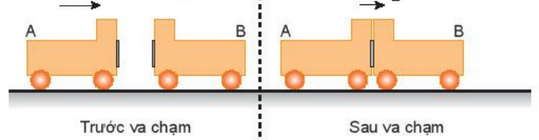
\includegraphics[scale=0.8]{../figs/G10-024-1}
\end{center}

Vật khối lượng $m_1$ chuyển động trên mặt phẳng ngang, nhẵn với vận tốc $\vec{v_1}$, đến va chạm với một vật khối lượng $m_2$ đang có vận tốc $v_2$. 

Sau va chạm, hai vật dính vào nhau, chuyển động với cùng một vận tốc $\vec{v}$.

Va chạm này gọi là va chạm mềm.

Áp dụng định luật bảo toàn động lượng:
\begin{equation*}
	m_1\vec{v}_1+ m_2\vec{v}_2 = (m_1+m_2)\vec{v}.
\end{equation*}
Suy ra 
\begin{equation*}
	\vec{v}=\dfrac{m_1\vec{v}_1+m_2\vec{v}_2}{m_1+m_2}.
\end{equation*}

\subsection{Vận dụng định luật bảo toàn động lượng đối với hai vật va chạm đàn hồi}

Vật khối lượng $m_1$ chuyển động theo chiều dương trên mặt phẳng ngang, nhẵn với vận tốc $\vec{v_1}$, đến va chạm với một vật khối lượng $m_2$ chuyển động ngược chiều dương với vận tốc $\vec{v_2}$. 

Sau va chạm, vật $m_1$ chuyển động ngược chiều dương với vận tốc $\vec{v_1'}$, vật $m_2$ chuyển động theo chiều dương với vận tốc $\vec{v_2'}$.

Va chạm được gọi là va chạm đàn hồi nếu không có sự biến dạng nào xảy ra trong quá trình va chạm. Trong va chạm đàn hồi, ngoài bảo toàn động lượng còn có thêm sự bảo toàn cơ năng. 

Để tìm trạng thái các vật sau va chạm, ta phải giải hệ gồm hai phương trình:
\begin{itemize}
	\item Phương trình bảo toàn động lượng 
	\begin{equation*}
		m_1\vec{v_1}+ m_2\vec{v_2} = m_1\vec{v_1'}+m_2\vec{v_2'}.
	\end{equation*}
	\item Phương trình bảo toàn cơ năng 
	\begin{align*}
		\dfrac{1}{2}m_1v_1^2+\dfrac{1}{2}m_2v_2^2=\dfrac{1}{2}m_1(v_1')^2+\dfrac{1}{2}m_2(v_2')^2
	\end{align*}
\end{itemize}
\luuy{
	Trong khi va chạm, lực tương tác giữa các vật va chạm được xem là lớn hơn rất nhiều so với tương tác giữa các vật đó với môi trường bên ngoài, do đó thế năng của các vật được bỏ qua, cơ năng của hệ chỉ gồm động năng các vật thành phần.
}
\subsection{Vận dụng định luật bảo toàn động lượng đối với chuyển động bằng phản lực}
\textbf{Bài toán: }Một tên lửa lúc đầu đứng yên, sau khi lượng khí với khối lượng $m$ phụt ra phía sau với vận tốc $\vec{v}$, thì tên lửa với khối lượng $M$ chuyển động với vận tốc $\vec{V}$.

Áp dụng định luật bảo toàn động lượng 
\begin{equation*}
	\vec{V}= - \dfrac{m}{M} \vec{v}.
\end{equation*}
\luuy{Tên lửa bay lên phía trước ngược với hướng khí phụt ra, không phụ thuộc vào môi trường bên ngoài là không khí hay chân không. Đó là nguyên tắc của chuyển động bằng phản lực.}
\ppgiai{
	\begin{description}
		\item[Bước 1] Xác định hệ cô lập, viết phương trình bảo toàn động lượng cho hệ cô lập (hệ kín):
		\begin{equation*}
			\vec{p_1}+\vec{p_2}+\vec{p_3}+ \ldots =\vec{p'_1}+\vec{p'_2}+\vec{p'_3}+ \ldots ;
		\end{equation*}
		\item [Bước 2] Thiết lập các phương trình hình chiếu trên các trục tọa độ O$x$ và O$y$:
		\begin{equation*}
			\begin{cases}
				p_{1x}+p_{2x}+p_{3x}+ \ldots &= p'_{1x}+p'_{2x}+p'_{3x}+ \ldots;\\
				p_{1y}+p_{2y}+p_{3y}+ \ldots &= p'_{1y}+p'_{2y}+p'_{3y}+ \ldots;
			\end{cases}
		\end{equation*}
		
		\item [Bước 3] Giải các phương trình hình chiếu, thu được giá trị đại lượng cần tìm.
		Trong một số trường hợp (va chạm đàn hồi) cần phải kết hợp thêm định luật bảo toàn năng lượng. 
	\end{description}
}

\section{Mục tiêu bài học - Ví dụ minh họa}
\begin{dang}{Áp dụng định luật bảo toàn động lượng trong các bài toán va chạm}
	\viduii{2}{Một vật khối lượng $m$ đang chuyển động theo phương ngang với vận tốc $v$ thì va chạm vào vật khối lượng $2m$ đang đứng yên. Sau va chạm, hai vật dính vào nhau và chuyển động với cùng vận tốc. Bỏ qua ma sát, vận tốc của hệ hai vật sau va chạm là
		\begin{mcq}(4)
			\item $\dfrac{v}{3}$. 
			\item $v$.
			\item $3v$.
			\item $\dfrac{v}{2}$.
		\end{mcq}
	}
	{	\begin{center}
			\textbf{Hướng dẫn giải}
		\end{center}
		Động lượng của hệ trước va chạm bằng tổng động lượng từng vật 
		\begin{align*}
			p_t=m_1v_1+m_2v_2=mv \qquad(v_2=0)
		\end{align*}
		Sau va chạm, hai vật dính vào nhau nên xem là một vật có khối lượng $m_1+m_2$ và có động lượng tương ứng là 
		\begin{align*}
			p_s=(m_1+m_2)v'=3mv'
		\end{align*}
		Áp dụng định luật bảo toàn động lượng 
		\begin{align*}
			p_t=p_s\quad\Rightarrow\quad mv=3mv'\quad\Rightarrow\quad v'=\dfrac{v}{3}.
		\end{align*}
		
		\textbf{Đán án: A}.
		
		\begin{center}
			\textbf{Câu hỏi tương tự}
		\end{center}
		
		Một vật khối lượng $m_1=\SI{1}{kg}$ chuyển động thẳng đều trên mặt phẳng nằm ngang với vận tốc $\SI{12}{m/s}$ và va chạm với vật có khối lượng $m_2=\SI{2}{kg}$ đang đứng yên. Sau va chạm, hai vật dính chặt với nhau. Bỏ qua mọi ma sát. Vận tốc của hai vật sau va chạm là
		\begin{mcq}(4)
			\item $\SI{4}{m/s}$. 
			\item $\SI{6}{m/s}$.
			\item $\SI{12}{m/s}$.
			\item $\SI{24}{m/s}$.
		\end{mcq}
		
		\textbf{Đáp án: A}.
	}
	\viduii{3}{Vật $m_1$ chuyển động với vận tốc $\SI{6}{\meter/\second}$ đến va chạm với vật $m_2$ chuyển động ngược chiều với vận tốc $\SI{2}{\meter/\second}$. Sau va chạm, hai vật bật ngược trở lại với cùng vận tốc $\SI{4}{\meter/\second}$. Tính khối lượng của hai vật biết $m_1+m_2=\SI{ 1,5}{\kilogram}$.
	}
	{	\begin{center}
			\textbf{Hướng dẫn giải}
		\end{center}
		
		Áp dụng định luật bảo toàn động lượng trong va chạm đàn hồi
		\begin{align*}
			m_1v_1 + m_2 v_2 &= m_1v_1' + m_2 v_2'\\ \Rightarrow\quad m_1\cdot\SI{6}{m/s} + m_2 \cdot \SI{-2}{m/s} &= m_1 \cdot \SI{-4}{m/s} + m_2 \cdot \SI{4}{m/s}\\
			\Rightarrow 10m_1-6m_2&=0
		\end{align*}
		Kết hợp với điều kiện $m_1+m_2=\SI{1.5}{\kilogram}$, ta giải được $m_1=\SI{0.5625}{\kilogram}$ và $m_2=\SI{0,9375}{\kilogram}$.
		
		
		\begin{center}
			\textbf{Câu hỏi tương tự}
		\end{center}
		
		Vật $\SI{200}{\gram}$ chuyển động với vận tốc $\SI{6}{\meter/\second}$ đến va chạm với vật $\SI{50}{\gram}$ chuyển động với vận tốc $\SI{4}{\meter/\second}$. Sau va chạm vật $\SI{200}{\gram}$ giữ nguyên hướng và chuyển động với vận tốc bằng nửa vận tốc ban đầu. Tính vận tốc của vật còn lại, biết rằng trước va chạm hai vật chuyển động ngược chiều.
		
		\textbf{Đáp án:} $v_2'=\SI{8}{m/s}$.
		
		
	}
\end{dang}

\begin{dang}{Áp dụng định luật bảo toàn động lượng \\trong bài toán chuyển động bằng phản lực}
	\viduii{2}{Một khẩu súng nằm ngang khối lượng $m_\text{s}=\SI{1000}{\kilogram}$, bắn một viên đạn khối lượng $m_\text{đ}=\SI{10}{\gram}$. Vận tốc viên đạn ra khỏi nòng súng là $\SI{600}{\meter/\second}$. Độ lớn vận tốc của súng sau khi bắn bằng là bao nhiêu?
	}
	{	\begin{center}
			\textbf{Hướng dẫn giải}
		\end{center}
		Chọn chiều dương là chiều chuyển động của đạn. 
		
		Trước khi bắn, hệ gồm súng và đạn không chuyển động nên có động lượng $p=0$.
		
		Sau khi bắn, hệ có động lượng 
		\begin{align*}
			p'=m_\text{s}v_\text{s}+m_\text{đ}v_\text{đ}
		\end{align*}
		Áp dụng định luật bảo toàn động lượng trước và sau khi bắn:
		\begin{align*}
			0 &= m_\text{s}v_\text{s} + m_\text{đ}v_\text{đ}'\\
			&= \SI{1000}{kg} \cdot v_\text s + \SI{0.01}{kg} \cdot \SI{600}{m/s}\\ 
			\Rightarrow\quad v_\text s &= \SI{-6e-3}{m/s}\\
			&=\SI{-6}{\milli\meter/\second}.
		\end{align*}
		Dấu trừ cho thấy súng bị giật ngược hướng chuyển động của đạn.
		
		
		\begin{center}
			\textbf{Câu hỏi tương tự}
		\end{center}
		
		Một khẩu súng nằm ngang khối lượng $m_\text{s} = 5\ \text{kg}$, bắn một viên đạn khối lượng $m_\text{đ} = 10\ \text{g}$. Vận tốc viên đạn ra khỏi nòng súng là 600 m/s. Độ lớn vận tốc của súng sau khi bắn bằng
		\begin{mcq}(4)
			\item 12 m/s.	
			\item 6 m/s.
			\item 1,2 m/s.	
			\item 60 m/s.
		\end{mcq}
		
		\textbf{Đáp án: C}.
	}
	\viduii{2}{
		Tên lửa có khối lượng vỏ là 10 tấn chuyển động với vận tốc $\SI{200}{\meter/\second}$ so với Trái Đất, 2 tấn khí phụt ra có vận tốc $\SI{500}{\meter/\second}$ so với tên lửa. Xác định vận tốc của tên lửa sau khi khí phụt ra.
	}
	{\begin{center}
			\textbf{Hướng dẫn giải}
		\end{center}
		
		Áp dụng định luật bảo toàn động lượng trước và sau khi khí phụt ra:
		$$(m_1+m_2)v = m_1v_1 + m_2 v_2$$ $$\Rightarrow (\SI{10000}{kg} + \SI{2000}{kg}) \cdot \SI{200}{m/s} = \SI{10000}{kg} \cdot v_1 + \SI{2000}{kg} \cdot (\SI{-500}{m/s})$$ $$\Rightarrow v_1  =\SI{340}{m/s}$$
		
		\begin{center}
			\textbf{Câu hỏi tương tự}
		\end{center}
		
		Tên lửa có khối lượng tổng cộng là 10 tấn chuyển động với vận tốc $\SI{200}{\meter/\second}$ so với Trái Đất, 2 tấn khí phụt ra có vận tốc $\SI{500}{\meter/\second}$ so với tên lửa. Xác định vận tốc của tên lửa sau khi khí phụt ra.
		
		\textbf{Đáp án:} $v_1  =\SI{375}{m/s}$.
	}
\end{dang}
\begin{dang}{Áp dụng định luật bảo toàn động lượng trong các bài toán đạn nổ}
	\viduii{2}{
		Một viên đạn khối lượng $\SI{0.5}{kg}$ đang bay theo phương ngang với vận tốc 1000 m/s thì nổ thành hai mảnh có khối lượng bằng nhau và cùng độ lớn vận tốc bay theo phương vuông góc với nhau. Xác định độ lớn động lượng của mỗi mảnh sau khi nổ.
	}
	{\begin{center}
			\textbf{Hướng dẫn giải}
		\end{center}
		
		\begin{itemize}
			\item Xét hệ gồm hai mảnh đạn trong thời gian nổ, đây được xem là hệ kín nên ta áp dụng định luật bảo toàn động lượng.
			\item Động lượng trước khi đạn nổ
			\begin{equation*}
				\vec{p}=m\vec{v} =\vec{p_{\text{t}}} 
			\end{equation*}
			\item Động lượng sau khi đạn nổ
			\begin{equation*}
				\vec{p_{\text{s}}}=m_1\vec{v_1}+m_2 \vec{v_2} =\vec{p_1} + \vec{p_2}. 
			\end{equation*}
			\item Vì hai mảnh sau khi nổ có động lượng bằng nhau và vuông góc với nhau nên
			\begin{equation*}
				p^2= p_1^2 + p_2^2 = 2p_1^2 \Rightarrow p = p_1 \sqrt{2} \Rightarrow p_1=p_2=\dfrac{p}{\sqrt{2}}=\SI{353.55}{kg \cdot m/s}.
			\end{equation*}
			
		\end{itemize}
		
		\begin{center}
			\textbf{Câu hỏi tương tự}
		\end{center}
		
		Một viên đạn khối lượng $\SI{1}{kg}$ đang bay theo phương ngang với vận tốc $100\sqrt 2$ m/s thì nổ thành hai mảnh có khối lượng bằng nhau và cùng độ lớn vận tốc, bay theo phương vuông góc với nhau. Xác định độ lớn động lượng của mỗi mảnh sau khi nổ.
		
		\textbf{Đáp án:} $\SI{100}{kg \cdot m/s}$.
	}
	\viduii{3}{Một viên đạn khối lượng 1 kg đang bay theo phương thẳng đứng với vận tốc 500 m/s thì nổ thành hai mảnh có khối lượng bằng nhau. Mảnh thứ nhất bay theo phương ngang với vận tốc 1000 m/s. Động lượng mảnh thứ hai có
		\begin{mcq}
			\item độ lớn $707\ \text{kg} \cdot \text{m/s}$; hướng lên trên tạo với phương ngang một góc $\beta= 60^\circ$.
			\item độ lớn $500\ \text{kg} \cdot \text{m/s}$; hướng lên trên tạo với phương ngang một góc $\beta= 60^\circ$. 
			\item độ lớn $500\ \text{kg} \cdot \text{m/s}$; hướng lên trên tạo với phương ngang một góc $\beta= 45^\circ$. 
			\item độ lớn $707\ \text{kg} \cdot \text{m/s}$; hướng lên trên tạo với phương ngang một góc $\beta= 45^\circ$.
		\end{mcq}
	}
	{	\begin{center}
			\textbf{Hướng dẫn giải}
		\end{center}
		
		\begin{center}
			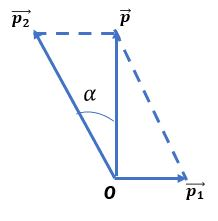
\includegraphics[scale=0.6]{../figs/VN10-PH-29-L-021-4-1.JPG}
		\end{center}
		Xét hệ gồm hai mảnh đạn trong thời gian nổ, đây được xem là hệ kín nên ta áp dụng định luật bảo toàn động lượng.
		
		Động lượng trước khi đạn nổ
		\begin{equation*}
			\vec{p}=m\vec{v} =\vec{p_{\text{t}}} 
		\end{equation*}
		
		Động lượng sau khi đạn nổ
		\begin{equation*}
			\vec{p_{\text{s}}}=m_1\vec{v_1}+m_2 \vec{v_2} =\vec{p_1} + \vec{p_2}. 
		\end{equation*}
		
		Áp dụng định luật bảo toàn động lượng
		\begin{align*}
			p_t=p_s \quad\Rightarrow\quad \vec{p}=\vec{p}_1+\vec{p}_2
		\end{align*}
		nên các vector động lượng có dạng như trên hình vẽ. Sử dụng định lý Pythagoras
		
		
		\begin{equation*}
			p^2_2 =p^2+p^2_1 \Rightarrow p_2  =\SI{707}{kg \cdot m/s}.
		\end{equation*}
		Góc giữa $\vec v_2$ và phương thẳng đứng: 
		\begin{equation*}
			\sin \alpha = \dfrac{p_1}{p_2} = \dfrac{1}{\sqrt 2} \Rightarrow \alpha = 45^\circ \Rightarrow \beta = 45^\circ.
		\end{equation*}
		
		\textbf{Đáp án: D.}
		
		\begin{center}
			\textbf{Câu hỏi tương tự}
		\end{center}
		
		Một viên đạn khối lượng $\SI{0.5}{kg}$ đang bay theo phương ngang với vận tốc 1000 m/s thì nổ thành hai mảnh có khối lượng bằng nhau. Mảnh thứ nhất bay theo phương thẳng đứng lên trên với vận tốc 1200 m/s. Động lượng mảnh thứ hai có
		\begin{mcq}
			\item độ lớn $464\ \text{kg} \cdot \text{m/s}$; hướng lên trên tạo với phương ngang một góc $\beta= 25^\circ$.
			\item độ lớn $464\ \text{kg} \cdot \text{m/s}$; hướng xuống dưới tạo với phương ngang một góc $\beta= 25^\circ$. 
			\item độ lớn $583\ \text{kg} \cdot \text{m/s}$; hướng lên trên tạo với phương ngang một góc $\beta= 31^\circ$. 
			\item độ lớn $583\ \text{kg} \cdot \text{m/s}$; hướng xuống dưới tạo với phương ngang một góc $\beta= 31^\circ$.
		\end{mcq}
		
		\textbf{Đáp án: D}.
	}
	
\end{dang}

\section{Trắc nghiệm}
\begin{enumerate}[label=\bfseries Câu \arabic*:]
	\item \mkstar{2}
	
	
	{
			Một vật khối lượng $m$ đang chuyển động theo phương ngang với vận tốc $v$ thì va chạm vào vật khối lượng $2m$ đang đứng yên. Sau va chạm, hai vật dính vào nhau và chuyển động với cùng vận tốc. Bỏ qua ma sát, vận tốc của hệ hai vật sau va chạm là
		\begin{mcq}(4)
			\item $\dfrac{v}{3}$. 
			\item $v$.
			\item $3v$.
			\item $\dfrac{v}{2}$.
		\end{mcq}
	}
	
	\hideall
	{	
		\textbf{Đáp án: A.}
		
		Áp dụng định luật bảo toàn động lượng trong va chạm mềm (hai vật dính vào nhau sau va chạm):
		$$m_1v_1 + m_2 v_2 = (m_1 + m_2) v \Rightarrow m v + 0 = 3m v' \Rightarrow v'=\dfrac{v}{3}.$$
	}
	\item \mkstar{2}
	
	
	{
		Một vật khối lượng $m_1=\SI{1}{kg}$ chuyển động thẳng đều trên mặt phẳng nằm ngang với vận tốc $\SI{12}{m/s}$ và va chạm với vật có khối lượng $m_2=\SI{2}{kg}$ đang đứng yên. Sau va chạm, hai vật dính chặt với nhau. Bỏ qua mọi ma sát. Vận tốc của hai vật sau va chạm là
		\begin{mcq}(4)
			\item $\SI{4}{m/s}$. 
			\item $\SI{6}{m/s}$.
			\item $\SI{12}{m/s}$.
			\item $\SI{24}{m/s}$.
		\end{mcq}
	}
	
	\hideall
	{	
		\textbf{Đáp án: A.}
		
		Áp dụng định luật bảo toàn động lượng trong va chạm mềm (hai vật dính vào nhau sau va chạm):
		$$m_1v_1 + m_2 v_2 = (m_1 + m_2) v \Rightarrow v=\SI{4}{m/s}.$$
	}
		\item \mkstar{2}
	
	
	{Một vật có khối lượng $m$ chuyển động với vận tốc $\SI{3}{m/s}$ đến va chạm với một vật có khối lượng  $2m$ đang đứng yên. Coi va chạm giữa hai vật là mềm. Sau va chạm, hai vật dính nhau và chuyển động với cùng vận tốc 
	
		\begin{mcq}(4)
			\item $\SI{2}{m/s}$. 
			\item $\SI{1}{m/s}$.
			\item $\SI{3}{m/s}$.
			\item $\SI{4}{m/s}$.
		\end{mcq}
	}
	
	\hideall
	{	
		\textbf{Đáp án: B.}
		
		Hệ hai vật ngay khi va chạm mềm là một hệ kín nên động lượng của hệ được bảo toàn:
		
		$$m_1\vec v_1 + m_2\vec v_2 = (m_1+m_2)\vec v.$$
		
		Do $v_2 = 0.$
		
		Suy ra:
		
		$$ v = \dfrac{m_1v_1}{m_1+m_2} = \dfrac{3m}{m+2m} = \SI{1}{m/s}.$$
		
	}
	\item \mkstar{2}
	
	
	{
		Một viên đạn đang bay với vận tốc $\SI{10}{m/s}$ thì nổ thành hai mảnh. Mảnh thứ nhất chiếm $60\%$ khối lượng của quả lựu đạn và tiếp tục bay theo hướng của vật với vận tốc $\SI{25}{m/s}$. Tốc độ và hướng chuyển động của mảnh thứ hai là 
		\begin{mcq}
			\item $\SI{12,5}{m/s}$; theo hướng viên đạn ban đầu. 
			\item $\SI{12,5}{m/s}$; ngược hướng viên đạn ban đầu.
			\item $\SI{6,25}{m/s}$; theo hướng viên đạn ban đầu. 
			\item $\SI{4}{m/s}$; ngược hướng viên đạn ban đầu.
		\end{mcq}
	}
	
	\hideall
	{	
		\textbf{Đáp án: B.}
		
		Hệ viên đạn (hai mảnh đạn) ngay khi nổ là một hệ kín nên động lượng hệ được bảo toàn
		
		$$m\vec v = m_1 \vec v_1 + (m-m_1)\vec v_2.$$
		
		Do $\vec v_1$ ngược chiều $v$.
		
		Nên 
		
		$$v_2 = \dfrac{mv - m_1v_1}{m-m_1} = -\SI{12,5}{m/s}.$$
		
		Dấu (-) chứng tỏ mảnh đạn thứ 2 sẽ chuyển động ngược chiều chuyển động ban đầu của viên đạn và mảnh đạn thứ nhất.
	}
		\item \mkstar{2}
	
	
	{Chiếc xe chạy trên đường ngang với vận tốc $\SI{20}{m/s}$ va chạm mềm vào một chiếc xe khác đang đứng yên và có cùng khối lượng. Biết va chạm là va chạm mềm, sau va chạm vận tốc hai xe là
		\begin{mcq}(2)
			\item $v_1 = 0; v_2 = \SI{10}{m/s}.$ 
			\item $v_1 = v_2 = \SI{5}{m/s}.$ 
			\item $v_1 = v_2 = \SI{10}{m/s}.$
			\item $v_1 = v_2 = \SI{20}{m/s}.$
		\end{mcq}
	}
	
	\hideall
	{	\textbf{Đáp án: C.}
		
		Áp dụng định luật bảo toàn động lượng cho lúc trước và sau va chạm ta có:
		
		$$\vec p_1 = \vec p_2 \Leftrightarrow m\vec v = 2m \vec v' \Leftrightarrow v = 2v' \Rightarrow v' = \dfrac{v}{2} = \SI{10}{m/s}.$$
		
		Suy ra:
		
		$$v_1 = v_2 = \SI{10}{m/s}.$$
	}
	\item \mkstar{2}
	
	
	{Một đầu đạn khối lượng $\SI{5}{g}$ được bắn ra khỏi nòng của một khẩu súng khối lượng $\SI{5}{kg}$ với vận tốc $\SI{500}{m/s}$. Nếu bỏ qua khối lượng của vỏ đạn thì vận tốc giật của súng là
		\begin{mcq}(4)
			\item $\SI{5}{cm/s}$. 
			\item $\SI{0,5}{m/s}.$ 
			\item $\SI{12}{m/s}.$
			\item $\SI{50}{cm/s}.$ 
		\end{mcq}
	}
	
	\hideall
	{
		\textbf{Đáp án: B.}
		
		Trước khi bắn: $p_0 = 0$.
		
		Sau khi bắn:
		
		$$m_\text{s}v_\text{s} + m_\text{đ}v_\text{đ} = 0.$$
		
		Suy ra $v_\text{s} = - \dfrac{m_\text{đ}v_\text{đ}}{m_\text{s}} = -\SI{0,5}{m/s}.$
		
	}
	\item \mkstar{2}
	
	
	{Khối lượng súng là $\SI{4}{kg}$ và của đạn là $\SI{50}{g}$. Lúc thoát khỏi nòng súng, đạn có vận tốc $\SI{800}{m/s}$. Vận tốc giật lùi của súng là
		\begin{mcq}(4)
			\item $\SI{6}{m/s}$. 
			\item $\SI{7}{m/s}$. 
			\item $\SI{10}{m/s}$. 
			\item $\SI{12}{m/s}$. 
		\end{mcq}
	}
	
	\hideall
	{	\textbf{Đáp án: C.}
		
		Chọn chiều dương là chiều chuyển động của viên đạn sau khi bắn: $p_\text{t} = 0.$
		
		$$p_\text{s} = m_2v_2 - m_1v_1 = 40 - 4v_1.$$
		
		Áp dụng định luật bảo toàn động lượng:
		
		$$p_\text{t} = p_\text{s} \Leftrightarrow 0 = 40 - 4v_1 \Rightarrow v_1 = \SI{10}{m/s}.$$ 
	}
	\item \mkstar{2}
	
	
	{Một hòn bi khối lượng $m$ đang chuyển động với vận tốc $v$ đến va chạm mềm vào hòn bi thứ 2 khối lượng $3m$ đang nằm yên. Vận tốc hai viên bi sau va chạm là
		\begin{mcq}(4)
			\item $\dfrac{v}{3}.$
			\item $\dfrac{v}{4}.$ 
			\item $\dfrac{3v}{5}.$
			\item $\dfrac{v}{2}.$
		\end{mcq}
	}
	
	\hideall
	{	
		\textbf{Đáp án: B.}
		
		Hệ hai vật ngay khi va chạm mềm là một hệ kín nên động lượng của hệ được bảo toàn:
		
		$$m\vec v = (m+ 3m)\vec V.$$
		
		$$ \Rightarrow V = \dfrac{mv}{m + 3m} = \dfrac{v}{4}.$$
	}
	\item \mkstar{3}
	
	
	{Một vật khối lượng $m$ đang chuyển động theo phương ngang với vận tốc $v$ thì va chạm vào vật khối lượng $4m$ đang đứng yên. Sau va chạm, hai vật dính vào nhau và chuyển động với cùng vận tốc. Bỏ qua ma sát, vận tốc của hệ sau va chạm là 
		\begin{mcq}(4)
			\item $\dfrac{v}{5}.$
			\item $v.$
			\item $5v.$
			\item $\dfrac{v}{2}.$
		\end{mcq}
	}
	
	\hideall
	{	
		\textbf{Đáp án: A.}
		
		Hệ hai vật ngay khi va chạm mềm là một hệ kín nên động lượng của hệ được bảo toàn:
		
		$$m\vec v = (m+ 4m)\vec V.$$
		
		$$ \Rightarrow V = \dfrac{mv}{m + 4m} = \dfrac{v}{5}.$$
	}
		\item \mkstar{2}
	
	
	{Một người có khối lượng $m_1=\SI{60}{kg}$ nhảy từ một chiếc xe có khối lượng $m_2 = \SI{80}{kg}$ đang chuyển động theo phương ngang với vận tốc $v = \SI{3}{m/s}$. Biết vận tốc nhảy của người đối với xe lúc chưa thay đổi vận tốc là $v_0 = \SI{4}{m/s}$. Vận tốc của xe sau khi người ấy nhảy ngược chiều đối với xe là
		\begin{mcq}(4)
			\item $\SI{6}{m/s}.$
			\item $\SI{5}{m/s}.$ 
			\item $\SI{4}{m/s}.$
			\item $\SI{3}{m/s}.$
		\end{mcq}
	}
	
	\hideall
	{	
		\textbf{Đáp án: A.}
		
		Khi người nhảy ngược chiều xe, ta có vận tốc ngược chiều nhau.
		
		$$\Rightarrow v' = v - v_0 = - \SI{1}{m/s}.$$
		
		Áp dụng định luật bảo toàn động lượng cho hệ gồm người và xe ban đầu và khi người nhảy là:
		
		$$\vec p = \vec p_1 + \vec p_2 \Rightarrow p = p_1 + p_2.$$
		
		$$\Leftrightarrow (m_1+m_2)v = m_1v'+m_2V \Rightarrow V = \SI{6}{m/s}.$$
		
		
	}
	
\end{enumerate}
\hideall
{
	\begin{center}
		\textbf{BẢNG ĐÁP ÁN}
	\end{center}
	\begin{center}
		\begin{tabular}{|m{2.8em}|m{2.8em}|m{2.8em}|m{2.8em}|m{2.8em}|m{2.8em}|m{2.8em}|m{2.8em}|m{2.8em}|m{2.8em}|}
			\hline
			1.A  & 2.A  & 3.B  & 4.B  & 5.C  & 6.B  & 7.C  & 8.B  & 9.A  & 10.A  \\
			\hline
			
		\end{tabular}
	\end{center}
}
\section{Tự luận}
\begin{enumerate}[label=\bfseries Câu \arabic*:]
	
	\item \mkstar{2}
	
	
	{
		Một khẩu súng nằm ngang khối lượng $m_\text{s}=\SI{1000}{\kilogram}$, bắn một viên đạn khối lượng $m_\text{đ}=\SI{10}{\gram}$. Vận tốc viên đạn ra khỏi nòng súng là $\SI{600}{\meter/\second}$. Tính độ lớn vận tốc của súng sau khi bắn.
	}
	
	\hideall
	{	
		Áp dụng định luật bảo toàn động lượng trước và sau khi bắn:
		$$m_1v_1 + m_2 v_2 = m_1v_1' + m_2 v_2' \Rightarrow v_\text s = \SI{-6e-3}{m/s}.$$
		
		Dấu $-$ chứng tỏ súng bị giật lùi.
	}
	\item \mkstar{2}
	
	
	{
		Tên lửa có khối lượng vỏ là 10 tấn chuyển động với vận tốc $\SI{200}{\meter/\second}$ so với Trái Đất, 2 tấn khí phụt ra phía sau có vận tốc $\SI{500}{\meter/\second}$ so với Trái Đất. Xác định vận tốc của tên lửa so với Trái Đất sau khi khí phụt ra.
	}
	
	\hideall
	{	
		Áp dụng định luật bảo toàn động lượng trước và sau khi khí phụt ra:
		$$(m_1+m_2)v = m_1v_1 + m_2 v_2 \Rightarrow v_1  =\SI{340}{m/s}.$$
	}
	\item \mkstar{2}
	
	
	{
		Một xe có khối lượng 5 tấn bắt đầu hãm phanh chuyển động thẳng chậm dần đều dừng lại hẳn sau $\SI{20}{\second}$ kể từ lúc bắt đầu hãm phanh, trong thời gian đó xe chạy được $\SI{120}{\meter}$. Tính động lượng của xe lúc bắt đầu hãm phanh.
	}
	
	\hideall
	{	
		Vận tốc của xe lúc bắt đầu hãm phanh, giải hệ phương trình:
		
		$$\begin{cases}
			2aS=v^2 - v_0^2 \\
			v=at+v_0
		\end{cases}
		\Rightarrow
		\begin{cases}
			2a\cdot 120 =0 - v_0^2 \\
			0=a\cdot 20 + v_0
		\end{cases}
		\Rightarrow v_0 = \SI{12}{m/s}
		$$
		
		Động lượng của xe lúc bắt đầu hãm phanh: $p=mv_0=\SI{60000}{kg.m/s}$.
	}
	\item \mkstar{2}
	
	
	{
		Vật $m_1$ chuyển động với vận tốc $\SI{6}{\meter/\second}$ đến va chạm với vật $m_2$ chuyển động ngược chiều với vận tốc $\SI{2}{\meter/\second}$. Sau va chạm, hai vật bật ngược trở lại với vận tốc $\SI{4}{\meter/\second}$. Tính khối lượng của hai vật biết $m_1+m_2=\SI{ 1,5}{\kilogram}$.
	}
	
	\hideall
	{	
			Ta có 
			
			$$m_1+m_2=\SI{ 1,5}{\kilogram}.$$
		
			Áp dụng định luật bảo toàn động lượng trong va chạm đàn hồi:
			
			$$m_1v_1 + m_2 v_2 = m_1v_1' + m_2 v_2' \Rightarrow m_1\cdot\SI{6}{} + m_2 \cdot \SI{-2}{} = m_1 \cdot \SI{-4}{} + m_2 \cdot \SI{4}{}.$$
		
		Giải hệ 2 phương trình trên, thu được
		$\begin{cases}
			m_1=\SI{0,5625}{\kilogram}\\
			m_2=\SI{0,9375}{\kilogram}.
		\end{cases}$
	}
	\item \mkstar{2}
	
	
	{
		Vật $\SI{200}{\gram}$ chuyển động với vận tốc $\SI{6}{\meter/\second}$ đến va chạm với vật $\SI{50}{\gram}$ chuyển động với vận tốc $\SI{4}{\meter/\second}$. Sau va chạm vật $\SI{200}{\gram}$ giữ nguyên hướng và chuyển động với vận tốc bằng nửa vận tốc ban đầu. Tính vận tốc của vật còn lại trong các trường hợp sau:
		\begin{enumerate}[label=\alph*)]
			\item Trước va chạm hai vật chuyển động cùng chiều.
			\item Trước va chạm hai vật chuyển động ngược chiều.
		\end{enumerate}
	}
	
	\hideall
	{	
		\begin{enumerate}[label=\alph*)]
			\item Trước va chạm hai vật chuyển động cùng chiều.
			
			Áp dụng định luật bảo toàn động lượng trong va chạm đàn hồi:
			$$m_1v_1 + m_2 v_2 = m_1v_1' + m_2 v_2' \Rightarrow v_2'=\SI{16}{m/s}.$$
			
			\item Trước va chạm hai vật chuyển động ngược chiều.
			
			Áp dụng định luật bảo toàn động lượng trong va chạm đàn hồi:
			$$m_1v_1 + m_2 v_2 = m_1v_1' + m_2 v_2' \Rightarrow v_2'=\SI{8}{m/s}.$$
		\end{enumerate}
	}
		\item \mkstar{2}
	
	
	{
		Một vật khối lượng $\SI{0.8}{kg}$ chuyển động trên mặt phẳng ngang với vận tốc $\SI{12}{m/s}$, đến va chạm với một vật khác có khối lượng $\SI{0.2}{kg}$ đang đứng yên trên mặt phẳng ngang ấy. Sau va chạm hai vật nhập lại làm một và chuyển động với cùng vận tốc. Tính vận tốc của hai vật sau va chạm.
	}
	
	\hideall
	{	
		Áp dụng định luật bảo toàn động lượng trong va chạm mềm (hai vật dính vào nhau sau va chạm):
		$$m_1v_1 + m_2 v_2 = (m_1 + m_2) v \Rightarrow v=\SI{9.6}{m/s}.$$
	}
	\item \mkstar{2}
	
	
	{
		Một vật khối lượng $\SI{0.6}{kg}$ chuyển động trên mặt phẳng ngang với vận tốc $\SI{12}{m/s}$, đến va chạm với một vật khác có khối lượng $\SI{0.4}{kg}$ đang đứng yên trên mặt phẳng ngang ấy. Sau va chạm hai vật nhập lại làm một và chuyển động với cùng vận tốc. Tính vận tốc của hai vật sau va chạm.
	}
	
	\hideall
	{	
		Áp dụng định luật bảo toàn động lượng trong va chạm mềm (hai vật dính vào nhau sau va chạm):
		
		$$m_1v_1 + m_2 v_2 = (m_1 + m_2) v \Rightarrow v=\SI{7.2}{m/s}.$$
	}
	\item \mkstar{2}
	
	
	{
		Một vật khối lượng $m_1=\SI{400}{g}$ chuyển động trên mặt phẳng ngang với vận tốc $\SI{18}{km/h}$, đến va chạm với một vật khác có khối lượng $\SI{100}{g}$ đang đứng yên trên mặt phẳng ngang ấy. Sau va chạm hai vật nhập lại làm một và chuyển động với cùng vận tốc. Tính vận tốc của hai vật sau va chạm.
	}
	
	\hideall
	{	
		Áp dụng định luật bảo toàn động lượng trong va chạm mềm (hai vật dính vào nhau sau va chạm):
		$$m_1v_1 + m_2 v_2 = (m_1 + m_2) v \Rightarrow v=\SI{4}{m/s}.$$
	}
		\item \mkstar{2}
	
	
	{
	Một khẩu súng $M = \SI{4}{kg}$ bắn ra viên đạn $m = \SI{20}{g}$. Vận tốc của đạn ra khỏi nòng súng là $\SI{600}{m/s}$. Súng giật lùi với vận tốc $V$ có độ lớn là bao nhiêu?
	}
	
	\hideall
	{	
		Chọn chiều dương là chiều chuyển động của viên đạn.
		
		Áp dụng bảo toàn động lượng:
		
		$$mv - MV = 0 \Rightarrow V = \dfrac{mv}{M} = \SI{3}{m/s}.$$
	}
		\item \mkstar{2}
	
	
	{Một tên lửa khối lượng tổng cộng $m_0 = 70$ tấn đang bay với $v_0= \SI{200}{m/s}$ đối với trái đất thì tức thời phụt ra lượng khí $m_2 = 5$ tấn, $v_2 = \SI{450}{m/s}$ đối với tên lửa. Tính vận tốc tên lửa sau khi phụt khí ra.
	}
	
	\hideall
	{	
		Theo định luật bảo toàn động lượng ta có:
		
		$$m_0v_0 = (m_0 -m)v' + m(v_0-v) \Rightarrow v' = \dfrac{m_0v_0 - m(v_0-v)}{m_0-m} \approx \SI{234,6}{m/s}.$$
	}
\end{enumerate}